\part{Requisitos Tecnol\'ogicos}
\section{Ferramentas de Codificação}

A game engine será a Unity3D que possuem suporte para multiplataforma, altamente otimizado, realiza renderizações e uma das características mais chamativas é que o Unity aceita três linguagens de programção, Boo, JavaScript e C\#, onde o C\# ser\'a usado como a linguagem de script para o projeto por ser bem parecido com o C e C++, facilitando assim o andamento da criação do jogo, pois os desenvolvedores j\'a possuem conhecimentos pr\'evios sobre as linguagens citadas. Os c\'odigos ser\~ao feitos dentro da própria game engine.


\section{Ferramentas de Modelagem}

A ferramenta para construir as cenas fazendo toda a modelagem 3D, também será o Unity3D. \'E um programa de f\'acil manipula\c{c}\~ao, devolve resultados extramente satisfat\'orios, bom sistema de anima\c{c}\~ao e o mais importante para o projeto é que existem vários pacotes prontos de cenas, objetos, personagens etc, disponíveis para uso.

\begin{figure}[!h]
	\centering
		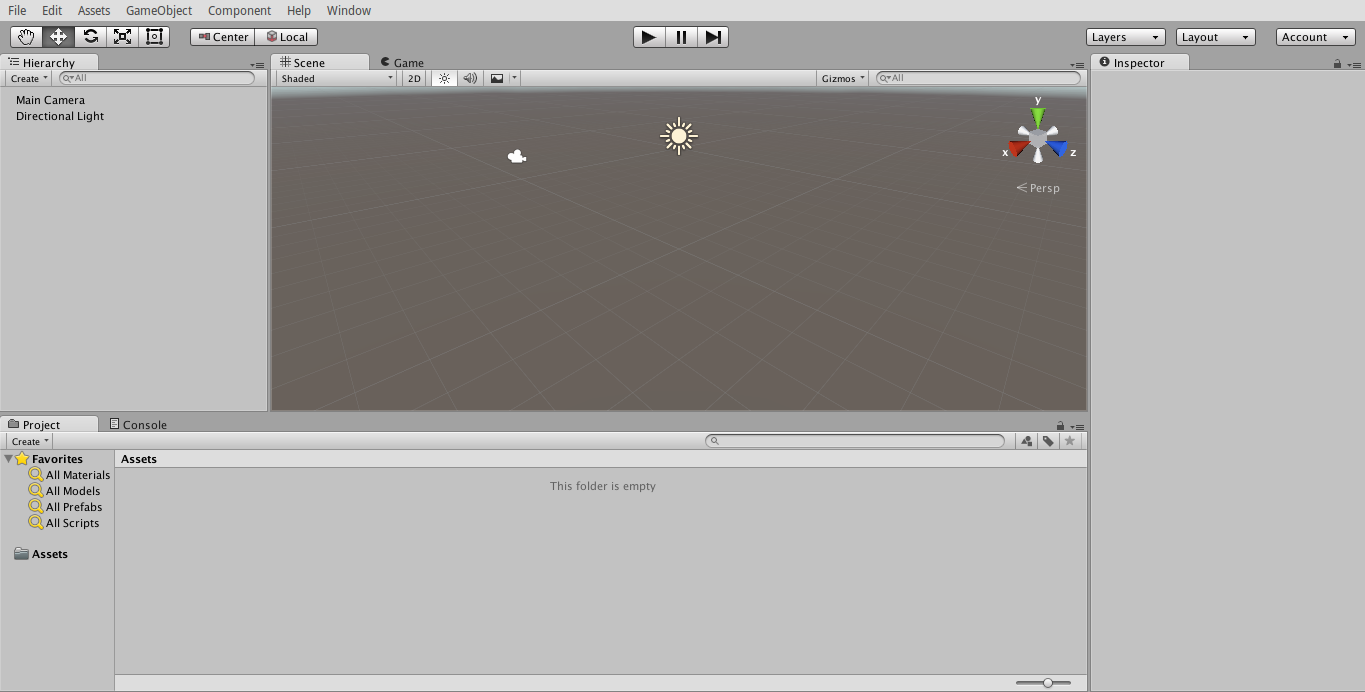
\includegraphics[scale=0.3]{figuras/unity}
	\caption{Interface Unity 3D}
\end{figure}